\subsection{Variation across deposits and cases}
The synthetic holdout distribution in Figure~\ref{fig:bs1-holdout} and Table~\ref{tab:learned-by-archetype} rules out describing this policy by its median alone. Porphyry cases retain higher ratios in this generator, while the vein group contains most observations below the fixed 0.90 diagnostic. These are paired generated cases, not independent geological samples. Figure~\ref{fig:bs1-failures} plots the below-threshold fraction for each group; it does not identify a deployable classifier because the case family label is a generator label unavailable in the real benchmark inputs.

\begin{figure}[p]\centering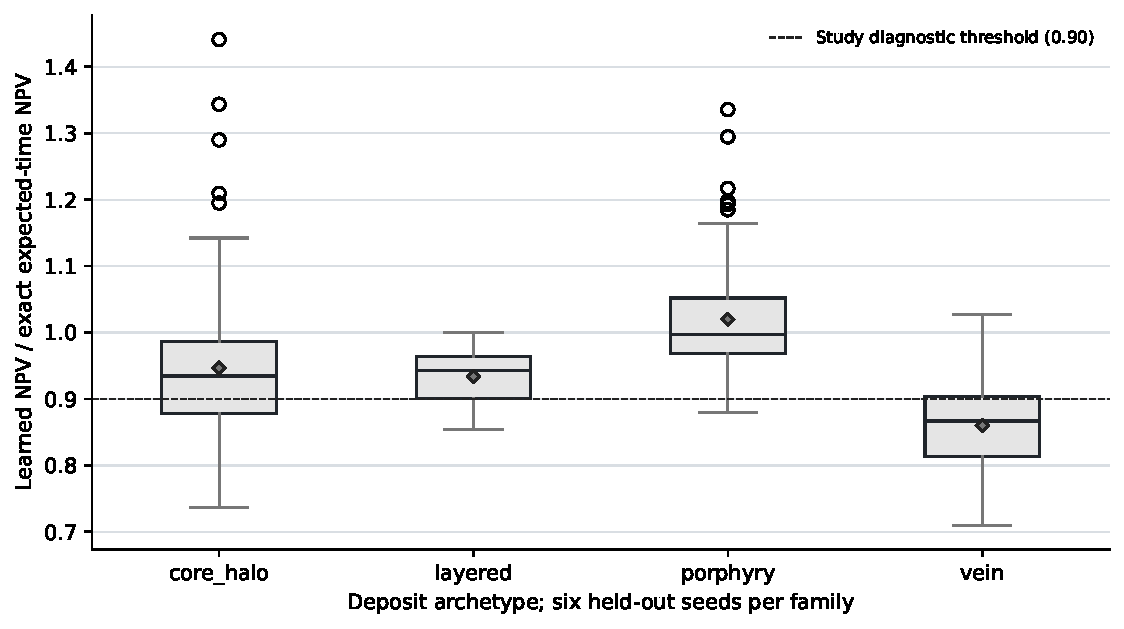
\includegraphics[width=0.86\textwidth,height=0.34\textheight,keepaspectratio]{figures/learned-holdout-by-archetype.pdf}\caption{Learned-to-exact schedule value ratios for unseen generated deposit seeds, stratified by family to expose variation hidden by the aggregate median.}\label{fig:bs1-holdout}\end{figure}
\begin{figure}[p]\centering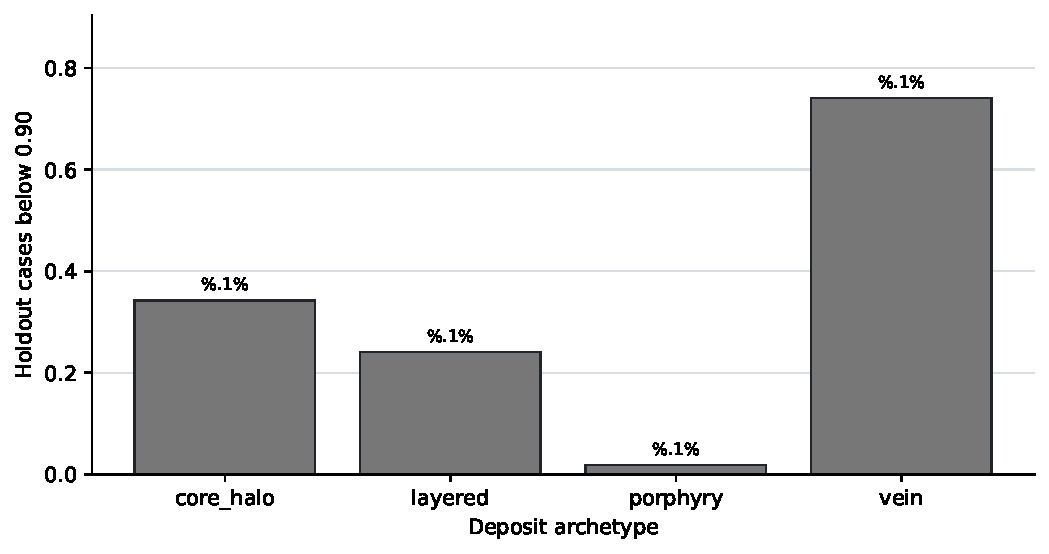
\includegraphics[width=0.82\textwidth,height=0.34\textheight,keepaspectratio]{figures/learned-failure-rate.pdf}\caption{Fraction of deposit-disjoint holdout cases below the 0.90 diagnostic ratio in each generated family, with the denominator shown in the accompanying table.}\label{fig:bs1-failures}\end{figure}

The two licensed benchmark results are plotted separately in Figure~\ref{fig:bs1-real} and enumerated in Table~\ref{tab:real-holdout}. Newman1 gives a ratio of 0.9989; KD gives 0.8987. This split result is evidence against a blanket transfer claim, and two instances are too few for an estimate of generalization error. The independent warning evaluation is summarized in Figure~\ref{fig:bs1-guard} and Table~\ref{tab:guard-validation}: the rule misses 76 cases below the diagnostic threshold, with measured precision 0.5278 and recall 0.4286. Figure~\ref{fig:bs1-guard-thresholds} shows that both required predictive thresholds are missed. The rule is unavailable as a live control, and the policy remains an ordering proposal rather than a certified optimization method.

\begin{figure}[p]\centering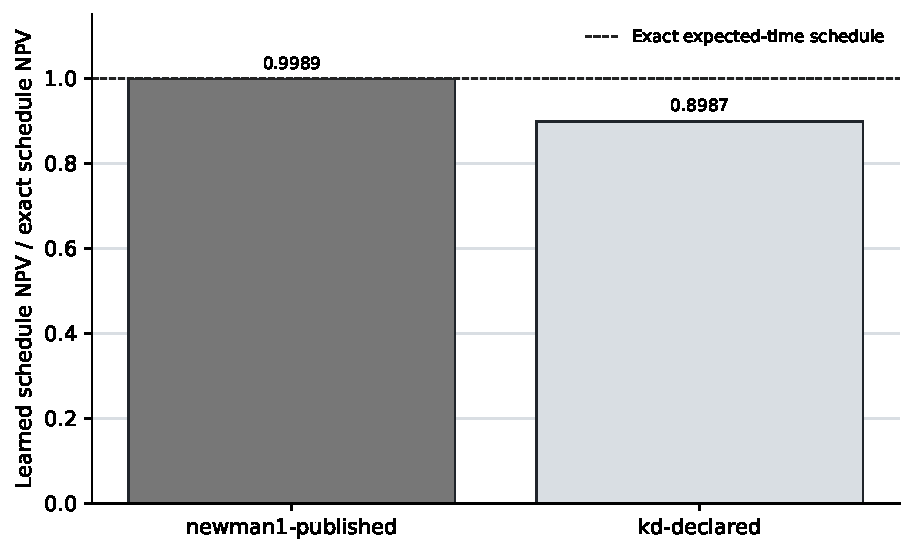
\includegraphics[width=0.72\textwidth,height=0.34\textheight,keepaspectratio]{figures/learned-real-holdout.pdf}\caption{The two MineLib learned-to-exact schedule value ratios are shown individually because their different outcomes cannot support a pooled transfer claim.}\label{fig:bs1-real}\end{figure}
\begin{figure}[p]\centering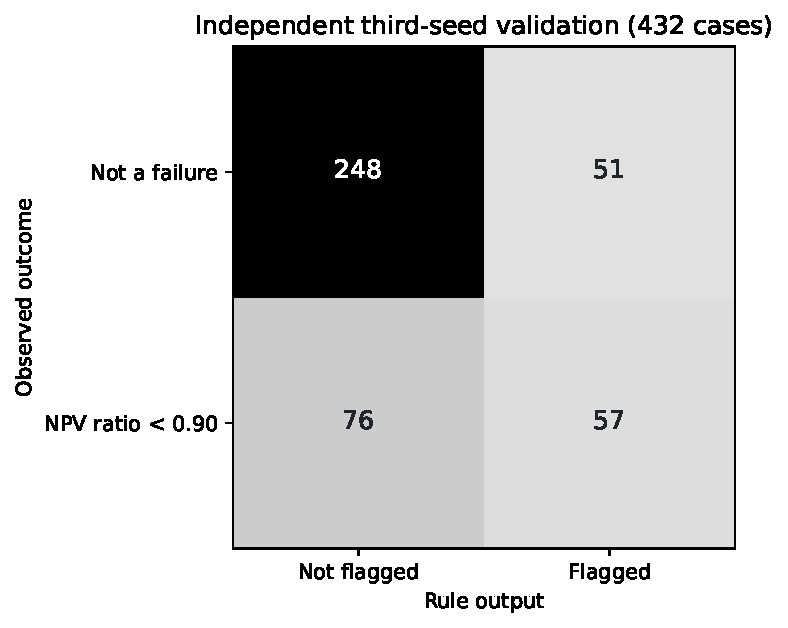
\includegraphics[width=0.68\textwidth,height=0.34\textheight,keepaspectratio]{figures/guard-confusion-matrix.pdf}\caption{Observed and predicted outcomes of the fixed warning rule on 432 third-split generated cases, showing false alarms and missed low-value schedules.}\label{fig:bs1-guard}\end{figure}
\begin{figure}[p]\centering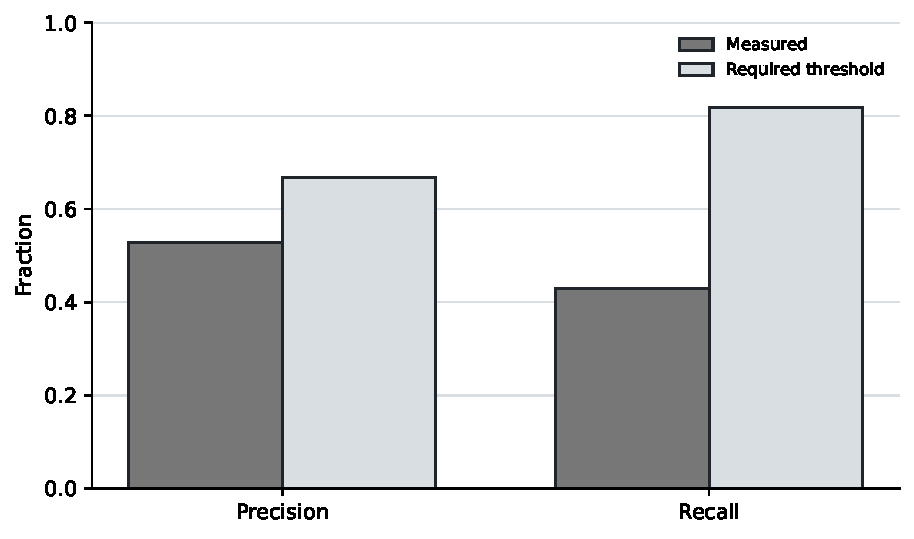
\includegraphics[width=0.72\textwidth,height=0.34\textheight,keepaspectratio]{figures/guard-thresholds.pdf}\caption{Measured precision and recall of the warning rule against the frozen minimum requirements, both of which the third-split evaluation fails.}\label{fig:bs1-guard-thresholds}\end{figure}

\begin{longtable}{lrrrrrr}
\caption{Deposit-disjoint synthetic evaluation results for the learned ordering and its exact comparator, grouped by archetype and measured on the same generated cases.}\label{tab:learned-by-archetype}\\
\toprule Archetype & $n$ & Median ratio & Mean ratio & 10th percentile & Minimum & Below 0.90 \\ \midrule
\endfirsthead\toprule Archetype & $n$ & Median ratio & Mean ratio & 10th percentile & Minimum & Below 0.90 \\ \midrule\endhead
core\_halo & 108 & 0.9348 & 0.9468 & 0.8482 & 0.7365 & 37/108 \\
layered & 108 & 0.9425 & 0.9337 & 0.8770 & 0.8536 & 26/108 \\
porphyry & 108 & 0.9972 & 1.0198 & 0.9484 & 0.8798 & 2/108 \\
vein & 108 & 0.8669 & 0.8600 & 0.7734 & 0.7101 & 80/108 \\
\bottomrule\end{longtable}

\begin{table}[htbp]\centering
\caption{The two licensed benchmark cases remain separate observations because they do not support an estimate of cross-deposit generalization.}\label{tab:real-holdout}
\begin{tabular}{lrrr}\toprule Case & Learned / exact ExTS & Spearman in pit & Scored \\ \midrule
newman1-published & 0.9989 & 0.2510 & yes \\
kd-declared & 0.8987 & 0.4214 & yes \\
\bottomrule\end{tabular}\end{table}

\begin{table}[htbp]\centering
\caption{The independently held-out warning rule is measured on 432 generated cases; the table preserves its false negatives and the thresholds it fails.}\label{tab:guard-validation}
\begin{tabular}{lrr}\toprule Measure & Measured & Required \\ \midrule
Precision & 0.5278 & $\geq 0.667$ \\
Recall & 0.4286 & $\geq 0.818$ \\
Worst unflagged ratio & 0.7322 & $\geq 0.7852$ \\
False negatives & 76 & 0 for complete detection \\
False positives & 51 & reported, not silently discounted \\
\bottomrule\end{tabular}\end{table}


\subsection{Computational cost}
Figure~\ref{fig:bs1-runtime} places the learned ordering among the methods recorded in the same case traces. The plot uses trace runtimes and a logarithmic scale; it mixes only method rows that are present and therefore does not establish a universal speedup. Exact expected-time ordering requires a relaxation solve, while the learned path performs feature extraction, five network evaluations, and the same feasibility-preserving constructor. In the current records, model inference is not the only runtime component. The comparison is a measured result for the registered cases, and a new engine or hardware configuration requires a fresh timing study.

\begin{figure}[p]\centering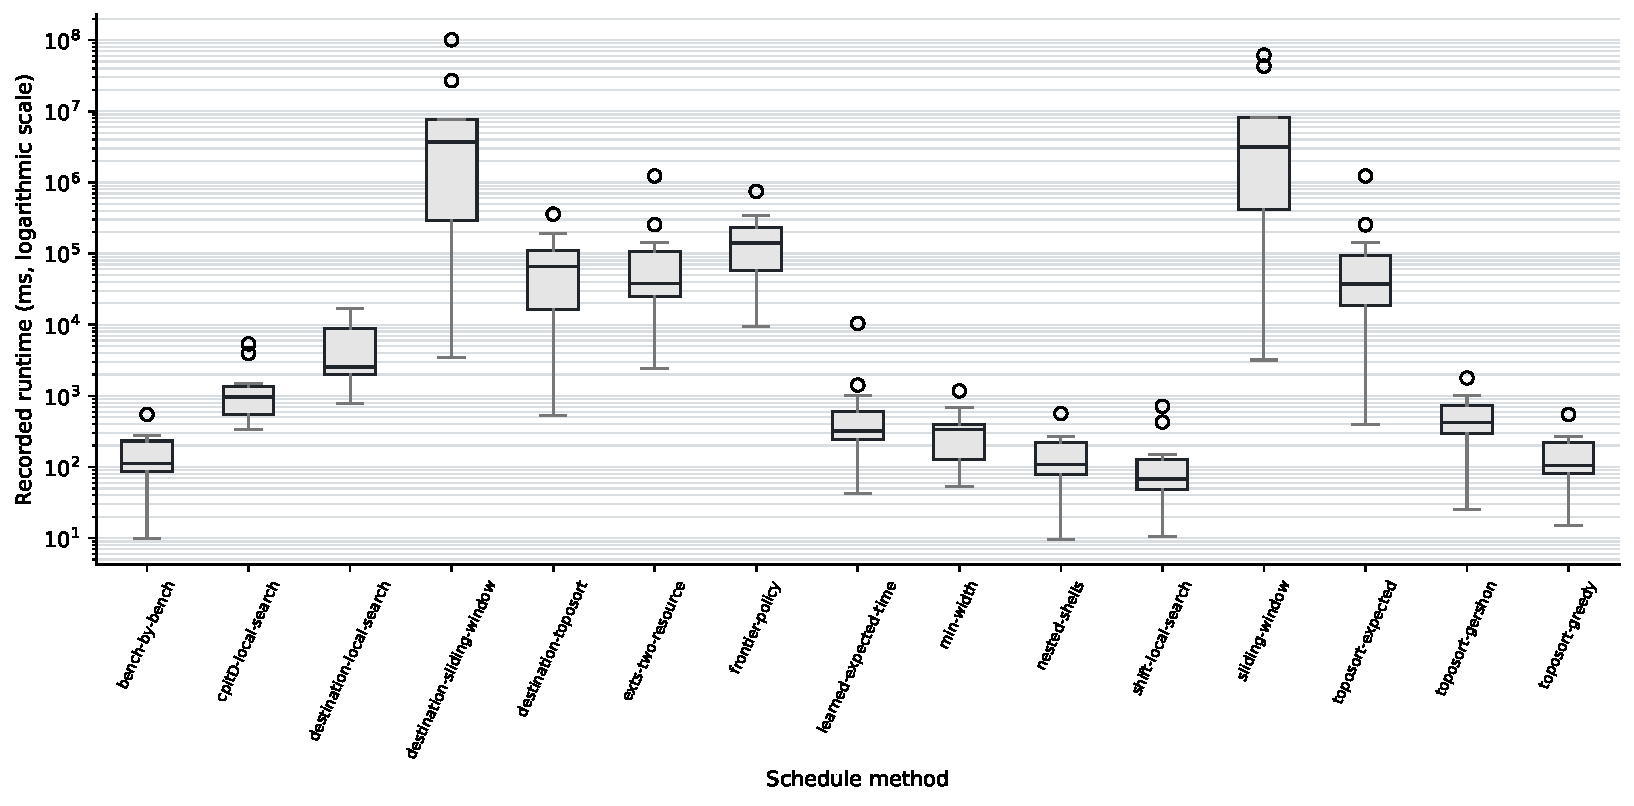
\includegraphics[width=\textwidth,height=0.34\textheight,keepaspectratio]{figures/method-runtime.pdf}\caption{Recorded runtime distributions for the learned policy and the other schedule methods across cases, with a logarithmic scale and no imputation for missing rows.}\label{fig:bs1-runtime}\end{figure}
